\documentclass[11pt]{book} 
\usepackage{amsmath, amsthm}
\usepackage{amssymb}
\usepackage{tikz}


\usepackage{xcolor}

\newcommand{\highlight}[1]{%
  \colorbox{yellow!50}{$\displaystyle#1$}}

\newtheorem{theorem}{Theorem}
\newtheorem{prop}{Proposition}


\newenvironment{definition}[1][Definition]{\begin{trivlist}
\item[\hskip \labelsep {\bfseries #1}]}{\end{trivlist}}
\newtheorem{example}{Example}


\usepackage{graphicx}
             % Book class in 11 points
\parindent0pt  \parskip10pt             % make block paragraphs
\raggedright                            % do not right justify

\title{\bf Open Calculus}    % Supply information
\author{Editor-in-chief: Adam Cross}   
          %   for the title page.
\date{\today}                           %   Use current date. 

% Note that book class by default is formatted to be printed back-to-back.
\begin{document}                        % End of preamble, start of text.
\frontmatter                            % only in book class (roman page #s)
\maketitle                              % Print title page.


\pagestyle{empty}
%% copyrightpage
\begingroup
\footnotesize
\parindent 0pt
\parskip \baselineskip

This work is subject to the GNU Free Documentation License (version 1.3) with the following additional clause: none of the major publishing houses may distribute this work commercially.

Complete license information is available at smartifybooks.com.

In particular, you may freely copy this work and you may distribute it for free or commercially (except major publishers), and you may edit this work to create your own fork of the project, but any such fork is subject to the same license.  


\vfill

Smartify Books, \\
Baton Rouge, LA \\
\texttt{smartifybooks.com}

%%%%{\LARGE\plogo}
\vspace*{2\baselineskip}


\endgroup
\clearpage








\tableofcontents                        % Print table of contents








\mainmatter                             % only in book class (arabic page #s)

\part{A Part Heading}                   % Print a "part" heading



\chapter{Limits}     



\section{Topology for Calculus, Lesson 1}



An ``open interval'' is an elementary idea.  We say an interval $(a,b)$ is open when it does not include its endpoints.  Now we define a more general notion of ``open''.  




\begin{definition}
A set $U$ in the real numbers is \emph{open} if for any element $x$ in $U$ there is an $\epsilon$ small enough so that $(x-\epsilon , x+\epsilon)$ is contained in $U$.  


\end{definition}



This is best illustrated with examples.  

\begin{example}
Is an ``open interval'' \emph{ open} according to this definition?  (If not, that would be really confusing, but let's make sure.)
\end{example}

Refer to the picture.  For any $x$ in the interval, you can find a small $\epsilon$ so that the small open interval $(x-\epsilon , x+\epsilon)$ is contained inside $(a,b)$.  
\begin{center}
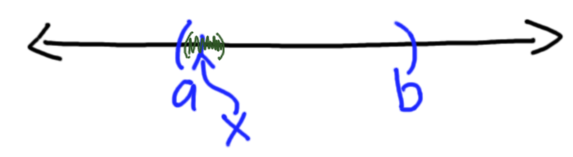
\includegraphics[width=4in]{toplec1_1.png}
\end{center}

So yes, intervals that are open in the ordinary sense are open in the sense we just defined.  


\begin{example}
Is a ``closed interval'' $[a,b]$ also \emph{open}?  Note that a closed interval includes its end points.

\end{example}

Here the answer is no because any open interval around $a$ no matter how small will contain values not in $[a,b]$.  It will contain some numbers less than $a$, and those are not in $[a,b]$.  There's a similar problem at $b$.  

\begin{center}
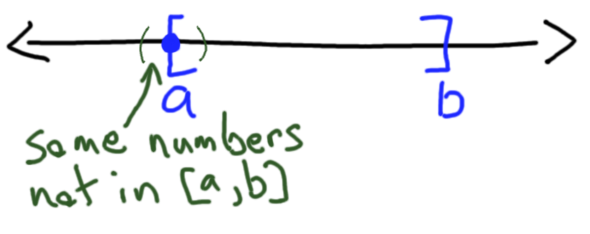
\includegraphics[width=4in]{toplec1_2.png}
\end{center}

\begin{example}
Is $(-1,1)\cup (3,4)$ open?  
\end{example}

Yes, a union of open intervals is open.

\begin{example}
Is the set $\mathbb{Z}$ of integers open?
\end{example}

No.  Any open interval around an integer contains numbers that are not integers.  Imagine a small interval around the number 1.  Students are sometimes tempted to say a set is ``closed'' when it is not open.  That's not correct.  We don't say a set is closed when it's not open.  In math, \emph{closed} has a different meaning.  


\begin{definition}
The \emph{preimage} $f^{-1}(U)$ is the set of all points $x$ where $f(x)$ is in $U$.
\end{definition}


Note that $f$ does not have to have an inverse, and here $f^{-1}$ does not mean the inverse in that sense, but they are related ideas.  When talking about preimages, we always put a \emph{set} inside $f^{-1}$, like $f^{-1}(U)$.

\begin{example}
Let $f(x)=\sin(x)$.  What is $f^{-1}(0,\infty)$?  Hint: This is exactly the same as asking to solve the inequality $f(x) >0$.
\end{example}


\begin{center}
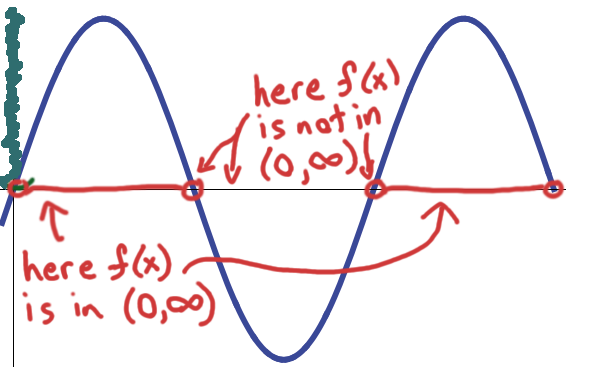
\includegraphics[width=4in]{toplec1_3.png}
\end{center}


In the picture I shaded $(0,\infty)$ along the y-axis.  In the picture we see $(0,\pi)$ and $(2\pi,3\pi)$ are both in $f^{-1}(0,\infty)$.  Those are both open intervals.  Since $\sin(x)$ just repeats the same wave over and over, 

$$f^{-1}(0,\infty) = \cdots (-4\pi,-3\pi)\cup (-2\pi,-\pi) \cup  (0,\pi) \cup  (2\pi,3\pi) \cup  (5\pi,6\pi) \cdots $$

This set $f^{-1}(0,\infty)$ is open.  It's an infinite union of open intervals.  


\begin{example}
Still considering $f(x)=\sin(x)$, what is $f^{-1}[0,1]$?  This is exactly the same as solving the inequality $0\leq f(x) \leq 1$.  
\end{example}

The only difference between this example and the last one is that now the preimage $f^{-1}[0,1]$ contains the end points.  

$$f^{-1}[0,1] = \cdots [-4\pi,-3\pi]\cup [-2\pi,-\pi] \cup  [0,\pi] \cup  [2\pi,3\pi] \cup  [5\pi,6\pi] \cdots $$

When we take an open set $U$, the preimage $f^{-1}(U)$ is also open.  This is true in general.

\begin{theorem}
If $f$ is continuous (everywhere) and $U$ is open, then $f^{-1}(U)$ is open.
\end{theorem}

This is an \textbf{equivalent} formulation of the idea of continuity.  It's a more mature way to understand continuity.  


Let's discuss the intuitive idea.  Below is a graph of a continuous function and an open set $U$.  By the picture, it certainly looks like $f^{-1}(U)$ is open, yes?  

\begin{center}
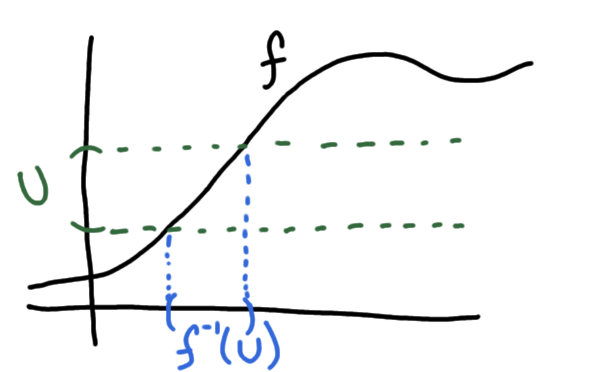
\includegraphics[width=4in]{toplec1_4.png}
\end{center}

Let's think a little about why it's open.  In the theorem, we do not assume that $U$ is an interval like in the picture.  To prove that $f^{-1}(U)$ is open, we need to show that for any $x$ in $f^{-1}(U)$ there is a little open interval around $x$ that is contained in $f^{-1}(U)$.

\begin{center}
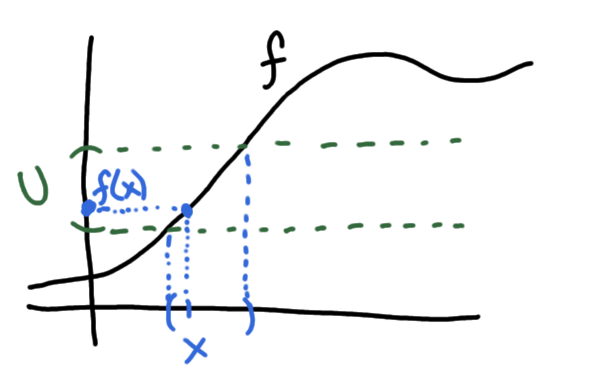
\includegraphics[width=4in]{toplec1_5.png}
\end{center}


An interval like that will look like this.  In the next image we see a little interval in red.  Any time a value $z$ is in that red interval, the function values $f(z)$ are inside $U$.  

\begin{center}
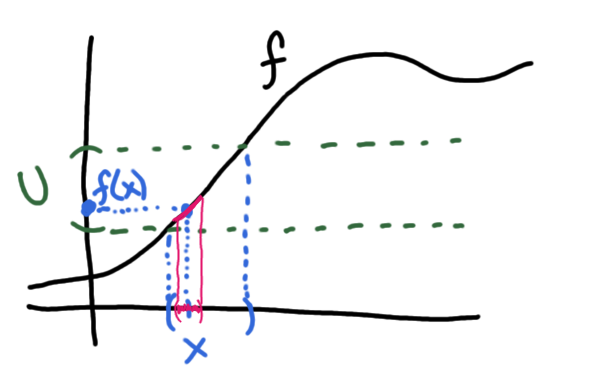
\includegraphics[width=4in]{toplec1_6.png}
\end{center}

Let's take one more step toward a formal proof.  Recall that $f(x)$ is in $U$ and $U$ is open.  That means we can produce a little open interval around $f(x)$ that is inside $U$.  In the next picture, we see a little $\epsilon$ interval $(f(x)-\epsilon, f(x)+\epsilon)$.  These are ``y''-values, so they are along the y axis.  

\begin{center}
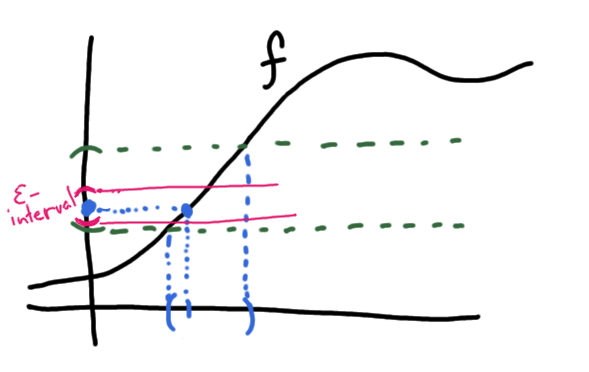
\includegraphics[width=4in]{toplec1_7.png}
\end{center}


Can we find a little $\delta$ interval around $x$ so that whenever $z$ is in  $(x-\delta,x+\delta)$ it follows that  $f(z)$ is in $(f(x)-\epsilon, f(x)+\epsilon)$?  If you are unsure, recall that this is exactly the definition of ``continuous at $x$''. 


\begin{center}
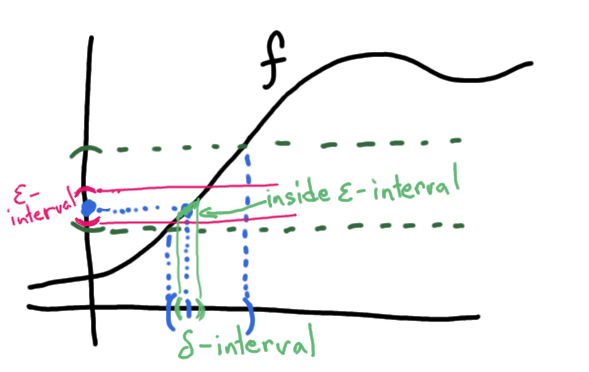
\includegraphics[width=4in]{toplec1_8.png}
\end{center}


If you understand this, then you will understand that the argument does not depend on our picture.  It works for any open set $U$.  


\subsection{The Role of Topology in Calculus}

Several of the most important ideas in calculus are basically topological---meaning to understand them the most natural thing is to use these ideas.  

Two of the most important examples: (1) the Intermediate Value Theorem, (2) the Extreme Value Theorem.


Here's why topology is useful in calculus.  So far we have defined everything \emph{pointwise}.  We defined continuity \emph{at x} and differentiability \emph{at x}, but some of the deeper theorems are about functions that are continuous \emph{everywhere}.  The Intermediate Value Theorem is not about any particular point, for example, and it's difficult to apply definitions of continuity that depend on some particular point $x$ when the theorem isn't about any particular point.  The alternative definition of continuous given in the theorem above allows us to take full advantage of functions that are continuous at every point in an interval.  

The ``topological'' method is an alternative point of view that will make the deeper theorems clearer if you can come to understand this point of view.  



\subsection{Exercises}

Ask me for help at the beginning of class or during office hours if you need help with these.



\begin{enumerate}
\item
Let $f(x)=\cos(x)$.  What is $f^{-1}(\{1\})$.  Here $\{1\}$ means the set containing just the number 1. Is $\{1\}$ open?  Is $f^{-1}(\{1\})$ open?




\item
Sketch an example of a function $f$ that is not continuous and some open set $U$ where $f^{-1}(U)$ is not open.  

\item
Refer to the theorem above about continuous functions.  If $U$ is not open, does that imply that $f^{-1}(U)$ is not open?

\item
Let $f(x)=x^2$.  Is $f$ continuous?  Let $U=(1,2)$. What is $f^{-1}(U)$?  Is $f^{-1}(U)$ open?  For this, don't just cite the theorem above, but convince yourself from the definition that it is open.



\end{enumerate}



\section{Exercises}

\begin{enumerate}

\item
Refer to the graphs.

\begin{center}
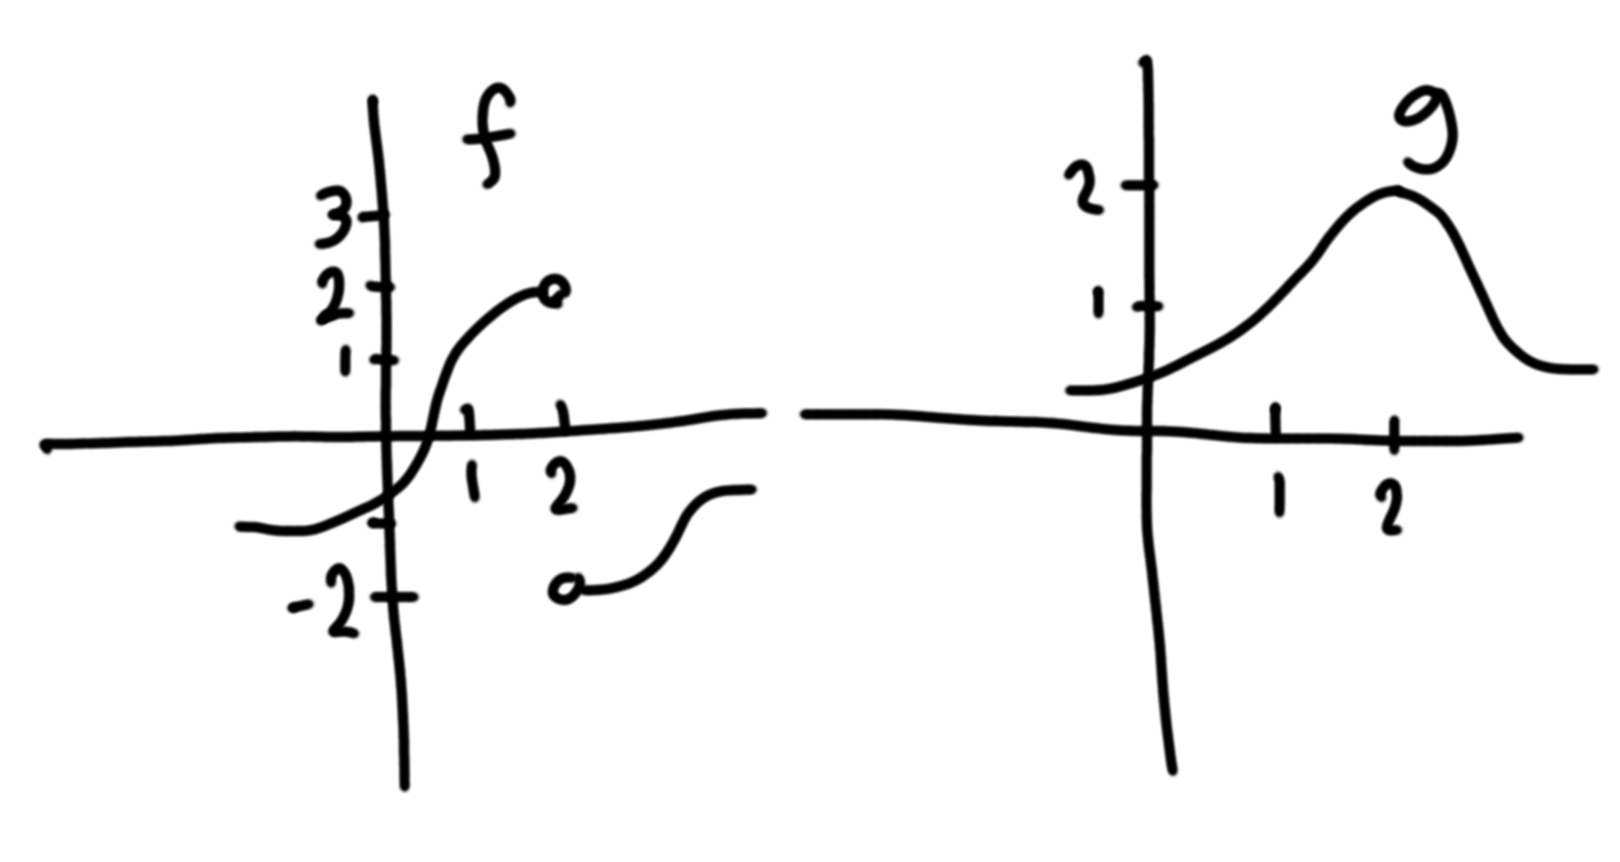
\includegraphics[width=4in]{limitExerciseImage1.png}
\end{center}

What is $\lim_{x\to 2} f(g(x))$?  What is $\lim_{x\to 2} g(f(x))$?




\item 

We will consider the limit $$\lim_{x\to 0} x^3.$$ 

\begin{enumerate}
\item 
Sketch a graph of $x^3$ around x=0 and draw two horizontal lines representing $\epsilon$ and $-\epsilon$. 



\item \label{b}
 What is the largest (most positive) value x can be so that   $x^3\leq \epsilon$?  
 

 
 \item \label{c}
  What is the most negative value x can be so that $x^3\geq -\epsilon$?



\item
What $\delta$ should we choose so that when $|x-0|<\delta$ we can be sure that $|x^3-0|<\epsilon$?  (Here we write the ``- 0'' part for emphasis so that it looks like the definition of a limit, but it can (and should) be omitted in most writing.  We want $\delta$ small so that $(x-\delta,x+\delta)$ is in the interval you identified in parts \ref{b} and \ref{c} above.



\item
If we require $|x^3-0|<1/1000$, how small does $|x|$ have to be?  



\end{enumerate}

\item

Explain in simple terms why $$\lim_{x\to 0} \frac{1}{x}$$ does not exist.  



\item
Explain in words why $$\lim_{x\to 0} x^2 \sin(2\pi/x)=0$$ (meaning the limit exists and is 0) but the limit $$\lim_{x\to 0} \sin(2\pi/x)$$ does not exist.  You are not required to write a proof, but explain what the essential difference is.









\end{enumerate}




\chapter{Derivatives}  





\section{The Chain Rule}


\begin{theorem}
If $f$ and $g$ are differentiable then $\frac{d}{dx}f(g(x)) = f'(g(x))g'(x)$.
\end{theorem}


The following proof sketch is intended to be illuminating rather than exactly precise.  An exactly precise proof would be written with $\epsilon$s and $\delta$s, but we think the student is more likely to undestand the idea presented this way.

\begin{proof}[Proof Sketch]

Since $g'(x)$ exists, for $h$ small, 
$$\frac{g(x+h)-g(x)}{h}\approx g'(x).$$

Here the $\approx$ symbol means ``is approximately''.  Therefore, 
$$g(x+h)-g(x)\approx hg'(x)$$
and 
$$g(x+h)\approx hg'(x)+g(x).$$

To compute the derivative of $f(g(x))$ at $x$, the difference quotient is $$\frac{f(g(x+h))-f(g(x))}{h}.$$
For $h$ small, 
$$ 
\frac{f(g(x+h))-f(g(x))}{h} \approx \frac{f(g(x) + hg'(x))-f(g(x))}{h}.$$
Observe we have just replaced $g(x+h)$ with $g(x) + hg'(x)$.  Next we multiply top and bottom by $g'(x)$ and we have 
\begin{equation} \label{3240972392408}
\frac{f(g(x) + hg'(x))-f(g(x))}{hg'(x)} g'(x).
\end{equation}

The quotient on the left in  (\ref{3240972392408}) almost has the form of a difference quotient.  As $h\to 0$, we also see that $hg'(x)\to 0$ so 
$$\lim_{h\to 0} \frac{f(g(x) + hg'(x))-f(g(x))}{hg'(x)}  = \lim_{h\to 0} \frac{f(g(x) + h)-f(g(x))}{h} = f'(g(x)).$$
Those limits are the same because it doesn't really matter what symbol appears in the highlighted portion of the difference quotient: 
$$\frac{f(g(x) + \highlight{hg\prime(x)})-f(g(x))}{\highlight{hg'(x)}}.$$
It only matters that those two numbers are the \emph{same} and that they are going to zero in the limit.  That's why we had to multiply and divide by $g'(x)$.  We needed to have the same number in those two highlighted positions.  

Thus $\frac{d}{dx}f(g(x)) = f'(g(x))g'(x)$.
\end{proof}

\section{Practice Quiz}

For the best learning experience, treat a practice quiz like an in-class quiz. Don't refer to other parts of the textbook.

\begin{enumerate}


\item Circle T for true or F for false:
\begin{enumerate}
\item T/F For any numbers $a$ and $b$, where $a<b$, there is a rational number $p/q$ so that $a<p/q<b$.

\item T/F The number $\sqrt{2}$ can be written as $p/q$ where $p$ and $q$ are both integers.

\item T/F The limit $\lim_{n\to \infty} (1+1/n)^{n}$ does not exist.

\item T/F It's possible to find a rational number as close to $\pi$ as you want.

\end{enumerate}


\item Compute the derivative.  

\begin{enumerate}
\item
$\frac{d}{dx} e^{\sin(x)}$
\item
$\frac{d}{dx} \ln(\cos(x))$
\item
$\frac{d}{dx} x^3\tan(x)$
\item
$\frac{d}{dx} \sin(x)^x$
\end{enumerate}




\item
Compute the derivative $\frac{d}{dx} \sin^{-1}(x)$ using the chain rule/implicit differentiation technique.  



\item Let's think about how to approximate $\sin(1^\circ)$.

\begin{enumerate}


\item  Since $1^\circ$ is close to $0^\circ$, we will find a tangent line at 0.  But why is $0^\circ$ any easier than $1^\circ$?



\item What is the slope of the tangent line at $0$?



\item What is the equation of the tangent line at $0$?



\item What is the value of the tangent line at $1^\circ$?  (Be sure to convert into radians.)



\item Why is your answer in the previous part a reasonable approximation to $\sin(1^\circ)$?

\end{enumerate}


\end{enumerate}



\section{Extreme Values}


We say a function $f$ has a \emph{local maximum} at a point $a$ if there is an interval $(a-\epsilon,a+\epsilon)$ around $a$ where $f(x)\leq f(a)$ for all $x$ in $(a-\epsilon,a+\epsilon)$ and in the domain of $f$. 

Another way to say this is $f(x)\leq f(a)$ in a neighborhood of $a$.  

A \emph{local maximum} is defined similarly.  


We say $f$ has a \emph{global maximum} at $a$ if $f(x)\leq f(x)$ for all $x$ in the domain of $f$.  

A \emph{global maximum} is defined similarly.  



\begin{prop}
If $f$ is defined on an interval $[a,b]$ and $f$ has a local minimum or a local maximum at $c \in [a,b]$, where $c$ is not one of the endpoints, and if $f$ is differentiable at $c$ then $f'(c)=0$.   
\end{prop}

Why did we assume $c$ isn't an endpoint?  Consider $f(x)=x^2$ restricted to the domain $[-2,2]$.  Then $f$ has a local (and global) max at $x=2$, but the derivative at $2$ is $f'(2)=4$.  

\begin{center}
\begin{tikzpicture}
  \draw[<->] (-3,0) -- (3,0) node[right] {$x$};
  \draw[<->] (0,-1) -- (0,4.2) node[above] {$y$};
\draw (-2,-0.1) -- (-2,0.1)
node[below=0.1in] {-2};
\draw (2,-0.1) -- (2,0.1)
node[below=0.1in] {2};
\node[color=blue] at (-2,4) {\textbullet};
\node[color=blue] at (2,4) {\textbullet};
\draw[scale=1,domain=-2:2,smooth,variable=\x,blue] plot ({\x},{\x*\x});
\end{tikzpicture}
\end{center}

Is it possible that $f$ has a local maximum at $a$ but $f'(a)$ doesn't exist?  Consider $f(x)=|x|$, which has a local minimum at 0, but $f'(0)$ does not exist.  So we have to assume $f'(a)$ exists.  

\begin{center}
\begin{tikzpicture}
  \draw[<->] (-3,0) -- (3,0) node[right] {$x$};
  \draw[<->] (0,-1) -- (0,3) node[above] {$y$};
\draw (-2,-0.1) -- (-2,0.1)
node[below=0.1in] {-2};
\draw (2,-0.1) -- (2,0.1)
node[below=0.1in] {2};
\node[color=blue] at (-2,2) {\textbullet};
\node[color=blue] at (2,2) {\textbullet};
\draw[scale=1,domain=-2:2,smooth,variable=\x,blue] plot ({\x},{abs(\x)});
\end{tikzpicture}
\end{center}

\begin{proof}
Assume $f$ has a local maximum at $c$.  We consider the limit of $\frac{f(c+h)-f(c)}{h}$ as $h\to 0$ from the right and from the left.  

If $h>0$ and $h$ is small enough, then 
$$\frac{f(c+h)-f(c)}{h}\leq 0.$$
Consider the slope of the secant line in the following illustration.

\begin{center}
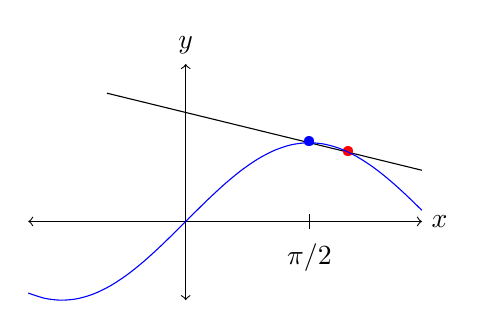
\begin{tikzpicture}
  \draw[<->] (-2,0) -- (3,0) node[right] {$x$};
  \draw[<->] (0,-1) -- (0,2) node[above] {$y$};

\draw (pi/2,-0.1) -- (pi/2,0.1)
node[below=0.1in] {$\pi/2$};

\draw (-1,1.629) -- (3,0.65);
\node[color=blue] at (pi/2,1) {\textbullet};
\node[color=red] at (2.07,.877) {\textbullet};
\draw[scale=1,domain=-2:3,smooth,variable=\x,blue] plot ({\x},{sin(\x r)});
\end{tikzpicture}
\end{center}

Thus $$\lim_{h\to 0^+}\frac{f(c+h)-f(c)}{h}\leq 0.$$

On the other hand, if $h<0$ then 
$$0\leq \frac{f(c+h)-f(c)}{h}.$$


\begin{center}
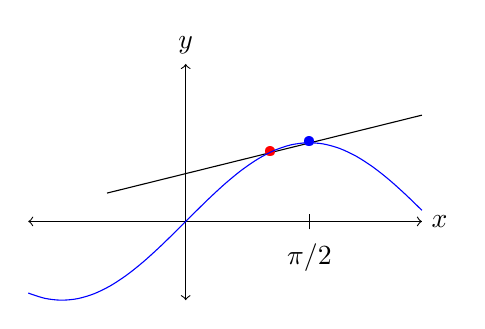
\begin{tikzpicture}
  \draw[<->] (-2,0) -- (3,0) node[right] {$x$};
  \draw[<->] (0,-1) -- (0,2) node[above] {$y$};

\draw (pi/2,-0.1) -- (pi/2,0.1)
node[below=0.1in] {$\pi/2$};

\draw (-1,.36) -- (3,1.35);
\node[color=blue] at (pi/2,1) {\textbullet};
\node[color=red] at (1.07,.877) {\textbullet};

\draw[scale=1,domain=-2:3,smooth,variable=\x,blue] plot ({\x},{sin(\x r)});
\end{tikzpicture}
\end{center}
Thus $$0\geq \lim_{h\to 0^-}\frac{f(c+h)-f(c)}{h}.$$
Since the limit exists, the right hand limit and the left hand limit are the same, so 
$$0\leq \lim_{h\to 0}\frac{f(c+h)-f(c)}{h} \leq 0$$
so $f'(c)=0$.

The argument is the same when $f$ has a local minimum at $c$.  The only difference is that the inequalities are flipped.  

\end{proof}








\chapter{Integrals}  



\end{document}                         